\documentclass{article}
\usepackage{amsmath, amssymb, mdwlist, graphicx, hyperref}
\usepackage{listings,color}
\usepackage{wrapfig}
\usepackage[usenames,dvipsnames]{xcolor}
\definecolor{gray}{rgb}{0.97,0.97,0.97}
\lstset{%
language=C,%
%backgroundcolor=\color{gray},
emph={putpixel},
emphstyle=\bf,
tabsize=4,
framesep=5pt,
mathescape=true,
xleftmargin=0.1cm,
xrightmargin=0.1cm,
frame=lines,
%basicstyle=\ttfamily,
%keywordstyle=\color{Blue},
%commentstyle=\color{OliveGreen},
%stringstyle=\color{MidnightBlue},
columns=flexible,
%showstringspaces=false
}

\newcommand{\mpar}[1]{\marginpar{\textit{#1}}}
\newcommand{\norm}[1]{\Vert #1 \Vert}
\DeclareMathOperator{\argmax}{argmax}
\DeclareMathOperator{\argmin}{argmin}
\newenvironment{solution}{\paragraph{Solution.}$\,$ }{\vskip 3mm\hrule}
\newenvironment{exercise}[2]{\paragraph{Exercise #1 (#2pt).} }{
\medskip}
\newcommand{\bbR}{\mathbb{R}}
\newcommand{\bw}{\mathbf{w}}
\newcommand{\bx}{\mathbf{x}}
\newcommand{\bd}{\mathbf{d}}
\newcommand{\bb}{\mathbf{b}}
\newcommand{\by}{\mathbf{y}}
\newcommand{\bzero}{\mathbf{0}}
\newcommand{\bz}{\mathbf{z}}
\newcommand{\bSigma}{\mathbf{\Sigma}}
\newcommand{\bp}{\mathbf{p}}
\newcommand{\bP}{\mathbf{P}}
\newcommand{\bm}{\mathbf{m}}
\newcommand{\bc}{\mathbf{c}}
\newcommand{\bM}{\mathbf{M}}
\newcommand{\bV}{\mathbf{V}}
\newcommand{\bK}{\mathbf{K}}
\newcommand{\bD}{\mathbf{D}}
\newcommand{\bA}{\mathbf{A}}
\newcommand{\bX}{\mathbf{X}}
\newcommand{\bY}{\mathbf{Y}}
\newcommand{\bR}{\mathbf{R}}
\newcommand{\bI}{\mathbf{I}}
\newcommand{\bS}{\mathbf{S}}
\newcommand{\bT}{\mathbf{T}}
\newcommand{\balpha}{\boldsymbol{\alpha}}
\newcommand{\pt}[2]{\left(\begin{array}{c}#1\\#2\end{array}\right)}

\begin{document}
\title{MTAT.03.015 Computer Graphics (Fall 2013)\\
Exercise session XIV: OGRE}
\author{Konstantin Tretyakov, Ilya Kuzovkin}
\date{December 9, 2013}
\maketitle

In this exercise session we will have a look at high-level graphics engine called OGRE\footnote{\url{http://www.ogre3d.org/}}. We will see how the concepts we know about are included into the OGRE engine, making our life easier: lighting, materials, shadows, environmental mapping and other techniques are made accessible by adding few lines of code, without the need to implement all annoying details on our own.

The solutions will have to be submitted as a zipped project directory. Please keep Windows libraries even if you work on Linux or Mac.

You can always seek for additional information and help in official tutorials \url{http://www.ogre3d.org/tikiwiki/tiki-index.php?page=Tutorials}.

\section{Structure of the application}
We start by comparing the structure of the application to the familiar structure we've been using so far. Please open \verb#1_OgreTriangle# project and read through the code in the \verb#triangle.cpp# file. Compare it to the GLUT-based applications we have seen before.

\begin{exercise}{1}{0.5}
Add a small square which will fly around the triangle and rotate around it's own center. For that you will need to
\begin{enumerate}
	\item Create new \verb#Ogre::ManualObject# object using \verb#createManualObject()# method of the scene manager.
	\item Describe vertices of your square. Look up in the documentation of the \\
\verb#Ogre::RenderOperation# class\footnote{\url{http://www.ogre3d.org/docs/api/html/classOgre_1_1RenderOperation.html}} which operation type you should use. Note that in OGRE we first create the vertex itself and then describe it's attributes.
	\item Create \verb#Ogre::SceneNode# and attach the new object to it.
	\item Use this \verb#SceneNode# to animate our object (update it's potision) in the \verb#frameRenderingQueued()# method, which is an analog of \verb#idleFunc()# in GLUT.
\end{enumerate}
The existing code for the triangle will serve you as example. The result should look something like this:
\begin{center}
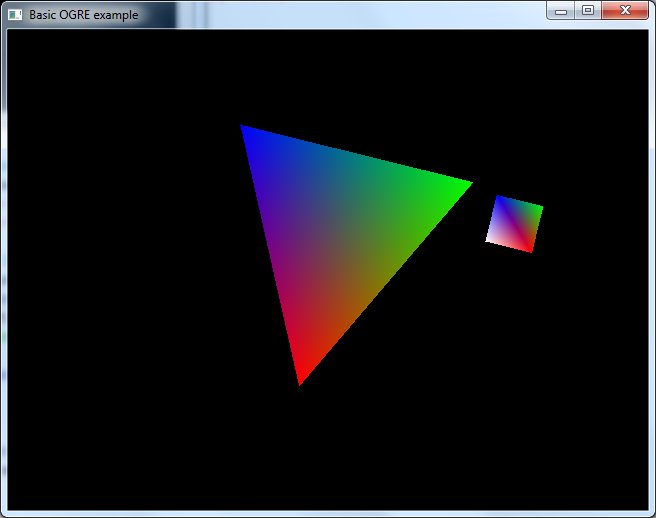
\includegraphics[width=0.7\textwidth]{ex1.png}
\end{center}
\end{exercise}

\section{Lighting, materials and textures}

Open project \verb#2_OgreLighting#. The structure is same as before. Have a look at \verb#createLitSphereScene()#, here we create a sphere, add materials to it and enable lighting. See how it is done. Now pay attention to these lines in the middle of  \verb#run()# function:
\begin{verbatim}
Ogre::ResourceGroupManager::getSingleton().
                     addResourceLocation("../data", "FileSystem");
Ogre::ResourceGroupManager::getSingleton().
                     initialiseAllResourceGroups();
\end{verbatim}
Instead of writing material properties into the code, materials (and some other things) can be described in special \emph{script} files. First line tells OGRE where to look for resources: various data files (textures, meshes, etc.) and scripts. Second line instructs it to read in resource descriptions and initialise \emph{resource groups}.

Have a look at the \verb#Examples.material# file in the \verb#data# folder and try to apply some of materials described there to our sphere:
\begin{verbatim}
sphere->setMaterialName("Examples/WaterStream");
\end{verbatim} 
If you would like to try other examples you should download Ogre SDK\footnote{\url{http://www.ogre3d.org/download/sdk}} and add the resources needed for each particular example to our \verb#data# folder.

\begin{exercise}{2}{0.5}
Create new file \verb#data/Sphere.material#. Here we will describe material for our sphere. Use \verb#data/Examples.material# and \url{http://www.ogre3d.org/docs/manual/manual_16.html} to create a material script, which exactly reproduces material parameters we have specified in the code. The result should look exactly the same: red sphere with white specular spot on it.
Note that you can use \verb#WASD# keys to move the camera and mouse to look around.
\end{exercise}

\begin{exercise}{3}{0.5}
In practice session \#9, which was about different types of shadows, we implemented three different shadow techniques. You might remember that for implementing stencil shadows you first needed to create shadow volume objects and after that implement the logic by carefully playing with stencil, color and depth buffers. OGRE allows you to enable stencil shadows with literally one line of code\footnote{See more \url{http://www.ogre3d.org/tikiwiki/tiki-index.php?page=Basic+Tutorial+2}}:
\begin{verbatim}
scene->setShadowTechnique(Ogre::SHADOWTYPE_STENCIL_ADDITIVE);
\end{verbatim}
Create a plane (\verb#Ogre::SceneManager::PT_PLANE#) below the sphere and enable shadows. Note that you can enable or disable whether specific object casts a shadow using \verb#setCastShadows()# method of \verb#Ogre::Entity# object.
\end{exercise}

\begin{exercise}{4}{0.5}
Next let's see how we can map textures on our objects. The best way to do that is, again, by using \verb#.material# scripts. Check out \verb#data/Examples.material# for examples. Note that you can create animated textures just by adding one line (for example see \verb#Examples/WaterStream#). Find your favourite picture in the internet and use it as texture for the plane.

Another popular use of texture is environmental mapping or cube mapping. Have a look at the tutorial\footnote{\url{http://www.ogre3d.org/tikiwiki/tiki-index.php?page=Basic+Tutorial+3}} and add SkyBox or SkyDome to our scene.
\end{exercise}

\begin{exercise}{5*}{0.5}
Look at the scene now. You might feel the urge to make sphere reflective. Study the code in \verb#examples/CubeMapping/include/CubeMapping.h#. Here is an approximate description of the steps you need to do:
\begin{enumerate}
	\item Make our \verb#Application# class inherit \verb#Ogre::RenderTargetListener#
	\item Make use of \verb#preRenderTargetUpdate()# method
	\item Add some global variables
	\item Create cube map texture in the same way as it is done in \verb#createCubeMap()#
	\item Use \verb#Examples/DynamicCubeMap# to create a new material in our \verb#Sphere.material# script
	\item Enable this material using \verb#setMaterialName()# method 	
\end{enumerate}
\end{exercise}
After completing exercises 3, 4 and 5 your scene will be something like this:
\begin{center}
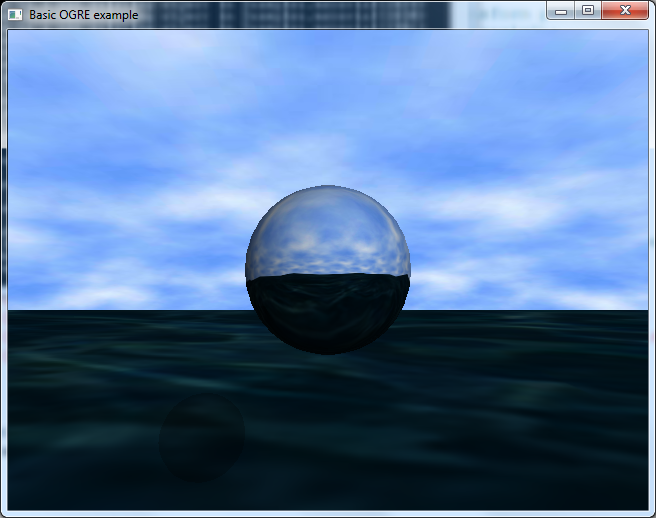
\includegraphics[width=0.7\textwidth]{ex3-4-5.png}
\end{center}



\section{Meshes and animations}

Now let us move to the next project and see how OGRE works with meshes. Open project \verb#3_OgreMesh#. Meshes are handles as any other object we have seen before: they are entities, have \verb#SceneNode# and you can specify materials and textures and shadows in the exactly same way as we have seen before. You can see that in \verb#setupBody()#.

The code you see in this project is rather complicated and represents simplified and adopted version of \verb#CharacterAnimation# OGRE sample application. You do not need to understand everything what is happening there, although it should not be hard.

\begin{exercise}{6}{0.5}
Currently our character is only able to run forward and swing sword on left mouse click (this does not work until you draw swords out, which you will need to implement). Add the following functionality (coding should happen inside keyboard and mouse listener section and in \verb#updateBody# method, you will see guiding comments in there):
\begin{enumerate}
	\item Enable movement in all four directions using \verb#WASD# keys
	\item Enable jumps on \verb#Spacebar#
	\item Draw swords on \verb#Q#
	\item On left mouse click the character swings sword vertically, but there is also horizontal swing animation available, make him do that on on right mouse click
	\item Do now allow character to run off the floor
\end{enumerate}
\begin{center}
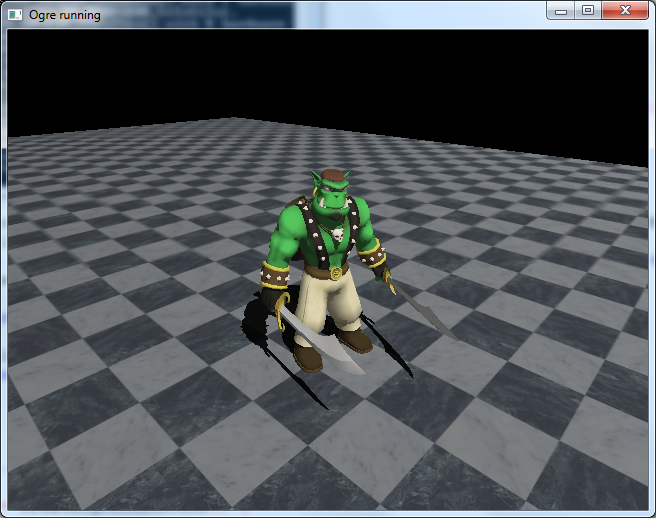
\includegraphics[width=0.7\textwidth]{ex6.png}
\end{center}
\end{exercise}


\begin{exercise}{7*}{2}
In OGRE official Basic Tutorial 3: ``Terrain, Sky, and Fog"\footnote{\url{http://www.ogre3d.org/tikiwiki/tiki-index.php?page=Basic+Tutorial+3}} you can learn how to create terrains, sky (as we already did in exercise 4) and fog. Like this:
\begin{center}
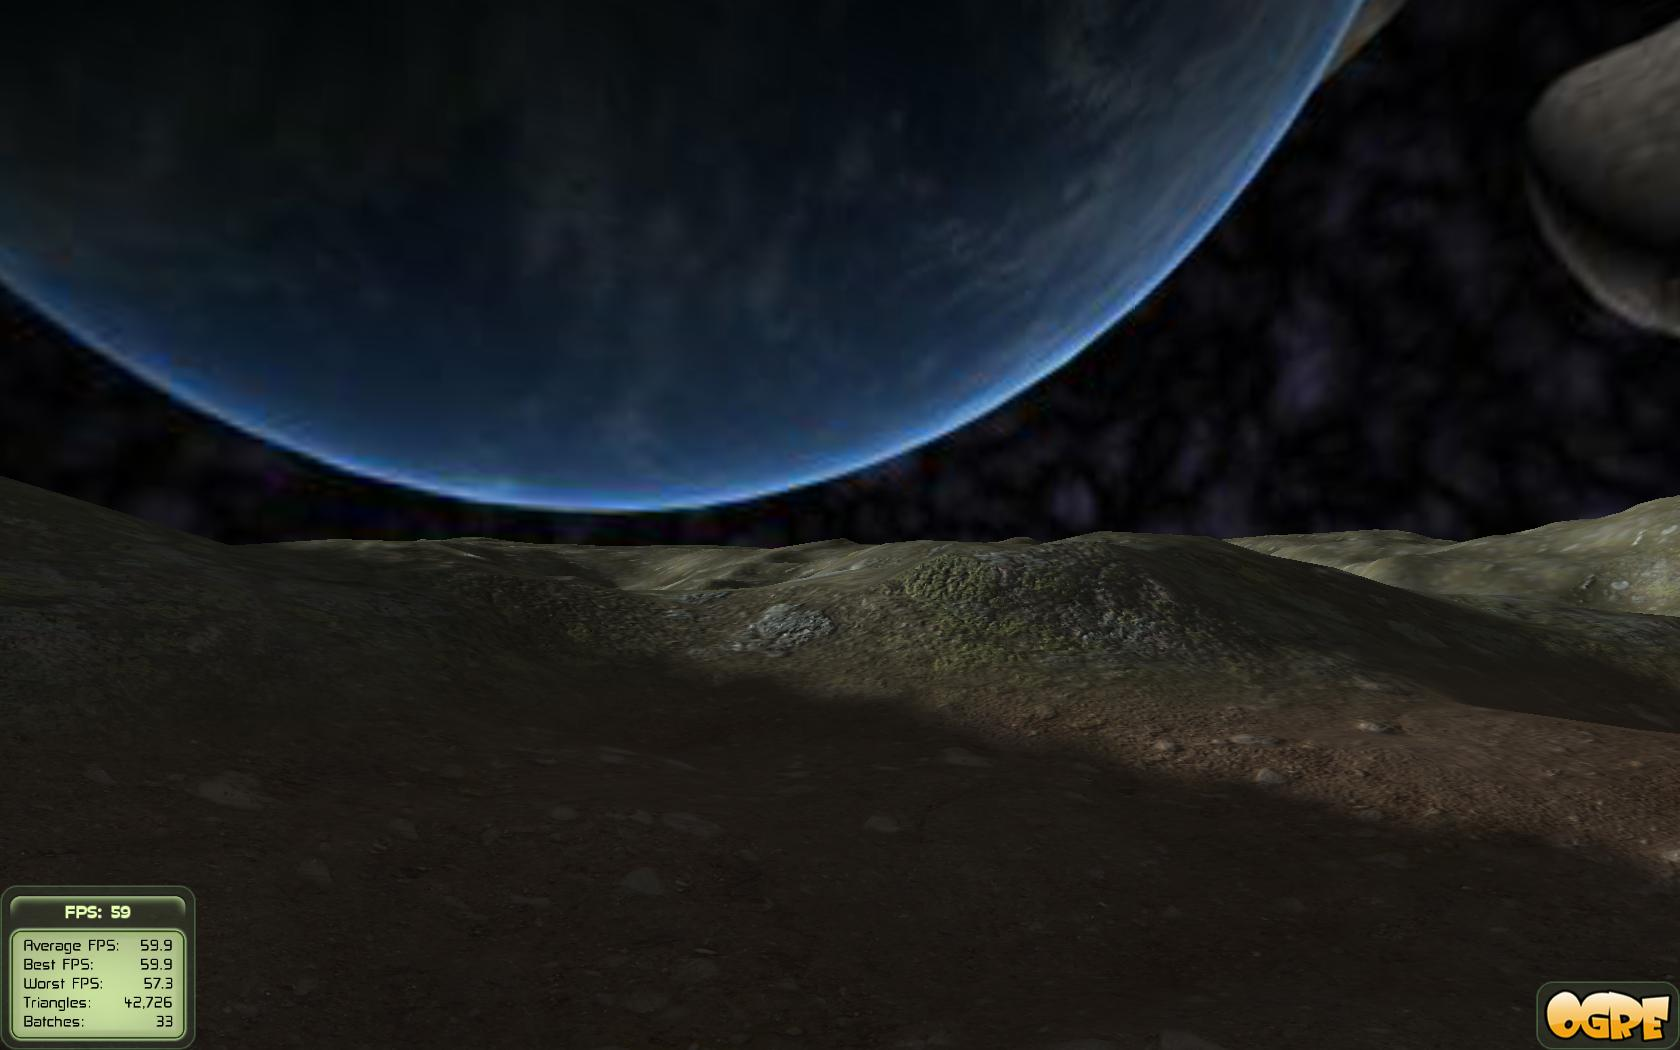
\includegraphics[width=0.7\textwidth]{terrain.jpg}
\end{center}
Take character from the previous exercise and place him into such world. Choose details to your own liking: terrain, sky, light, shadows, textures, reflections, army of ogres, another creatures\footnote{Look inside \texttt{media/models} folder of OGRE SDK for more meshes and characters}, mysterious reflective spheres in the middle of everything...
\end{exercise}


\section{Plugins}
In OGRE you can get additional functionality by using plugins. Open project \verb#4_OgrePlugins#. Have a look at the following line in the beginning of \verb#run# function:
\begin{verbatim}
mRoot = new Ogre::Root("plugins.cfg");
\end{verbatim}
It tells OGRE name of the file in \verb#bin# directory where plugin configuration resides. Inside that file you will see how we enable plugin called ParticleFX. This plugin has a configuration file, which resembles \verb#.material# files we have seen before. Open \verb#data/Examples.particle# and study it.

\begin{exercise}{8}{0.5}
To complete this exercise do the following:
\begin{enumerate}
	\item Make particle source follow mouse movements. For that you will need to add mouse listener in the way analogous to the way how keyboard listener is added. See helpful comments in the code.
	\item Play with different examples and their parameters, make the one you like best and describe it in new \verb#.particle# file.
\end{enumerate}
\end{exercise}


\end{document}
